\chapter{XML - eXtensible Markup Language}
In questo capitolo verrà descritto il linguaggio XML. Partendo dalla sua storia, dall'idea di partenza alle successive evoluzioni che hanno portato allo standard attuale, si illustreranno le caratteristiche che lo contraddistinguono, la sintassi e la semantica. Verranno introdotti anche gli strumenti necessari per definire e manipolare un documento XML come DTD, XSD e XPath. In conclusione una piccola parentesi su XML e il modello relazionale.

\section{Breve Storia di XML}
La storia di \textbf{XML} \emph{(eXtensible Markup Languages)} inizia negli anni '70 con lo sviluppo di \textbf{SGML} \emph{(Standardised Generalised Markup Language)} da parte di  Charles Goldfarb, insieme a Ed Mosher e Ray Lorie mentre lavoravano per IBM (Anderson, 2004). SGML a dispetto del nome non è propriamente un linguaggio di markup, ma piuttosto un linguaggio usato per specificare linguaggi di markup. Lo scopo di SGML era quello di creare vocabolari da poter usare nel markup di documenti con tag strutturati. Si immaginava all'epoca che certi documenti leggibili dalle macchine dovessero restare tali per decenni.
\\
Una delle applicazioni più popolare di SGML arrivò con lo sviluppo di \textbf{HTML} \emph{(HyperText Markup Language)} da parte di Tim Berners Lee alla fine degli anni '80 (Raggett, Lam, Alexander, Kmiec, 1998). Fin dal suo sviluppo HTML divenne in qualche modo vittima della propria popolarità,venendo rapidamente adottato ed esteso in molti modi oltre la visione originale.\\ Resta popolare tutt'oggi come tecnologia di presentazione ma è considerato inadatto come formato generico per immagazzinare dati. Quando si tratta di scambiare e immagazzinare dati HTML è una cattiva scelta, essendo originariamente indirizzato alla presentazione, mentre SGML è considerato troppo complicato per l'uso comune.
\\
XML riempe questa lacuna risultando leggibile sia alle macchine che alle persone, restando flessibile abbastanza da supportare scambi di dati indipendenti dalla piattaforma e dall'architettura.
Alla base, XML permette ad un ingegnere del software di creare un vocabolario e di utilizzarlo per descrivere dei dati. Ad esempio, nello scambio di dati tra computer, il numero 42 non è significativo a meno che non si trasmetta pure il significato dei dati, come la temperatura del processore espressa in gradi Celsius.
\\
Solo quando mittente e destinatario sono in accordo sul significato dei dati possono farne qualcosa di utile. Prima dello sviluppo di XML,
era in qualche modo necessario un accordo tra sistemi a priori sui dati e il loro significato. Con lo sviluppo di XML i dati possono essere scambiati senza accordi precedenti fintanto che entrambi i sistemi dispongano dello stesso vocabolario, ossia, parlino lo stesso linguaggio.
\\
Dallo sviluppo di XML sono emerse diverse applicazioni nelle seguenti aree:
\begin{description}
\item[Pubblicazioni Web:] XML permette di creare pagine interattive, dando possibilità di personalizzazione al cliente e rende la creazione di applicazioni di e-Commerce più intuitivo.
\item[Ricerche Web e automazione:] XML definisce il tipo di  informazione contenuto in un documento, rendendo più facile la restituzione di risultati utili durante le ricerche Web.
\item[Applicazioni Generiche:] XML fornisce un metodo standard per l'accesso alle informazioni, rendendo più facile ad applicazioni e dispositivi di ogni tipo  utilizzare, conservare, trasmettere e presentare dati.
\item[Applicazioni e-Business:] Implementazioni XML rendono l'\emph{Electronic Data Interchange} (EDI) più accessibile per lo scambio di informazioni, le transazioni tra azienda e azienda e le transazioni tra azienda e consumatore.
\item[Metadata Applications:] XML rende più semplice esprimere metadati in un formato portabile e riusabile.
\item[Computing Pervasivo:] XML fornisce tipi di dati portabili e strutturati da presentare su dispositivi pervasivi (wireless) come notebook, tablet e smartphone.
\end{description}
\section{Struttura e Sintassi}
Tutti i documenti XML sono formati da elementi rappresentati da due tag, uno di apertura e uno di chiusura, gli elementi possono contenere dati, altri elementi, una combinazione dei due, o nessuno di essi(elementi vuoti). I Documenti iniziano con un unico elemento radice che contiene sotto-elementi, i loro sotto-elementi e cosi via. Questo risulta in una struttura gerarchica ad albero all'interno del documento.\\\\
\begin{flushleft}
\begin{example}
Ecco un esempio di codice XML\\
\inputminted[linenos,frame=lines]{xml}{esempio1.xml}
\label{lst:xml_example}
\end{example}
\end{flushleft}

\subsection{Definire la struttura dei dati: DTD e XSD}
Pur essendo possibile intuire la struttura dei dati rappresentati leggendo il documento XML a volte è necessario definire una struttura rigida che vada rispettata; ci sono vari modi di ottenere questo, i più comuni sono \emph{Data Type Definition} (DTD) e \emph{XML Schema Definition} (XSD).

\paragraph{DTD - Data Type Definition:}DTD fu introdotto durante lo sviluppo di SGML ed è per questo motivo più indicato per applicazioni indirizzate ai documenti, come HTML. HTML infatti è specificato usando DTD. Basato sulla \emph{Extended Backus-Naur Form} (EBNF) può definire la struttura di un documento ma non ha l'abilità di specificare regole da applicare ai dati. Ovvero tutti i dati contenuti all'interno del documento vengono trattati dal DTD come una stringa. Questo si adatta ai linguaggi di markup per documenti, ma non è conveniente quando un'applicazione necessita il controllo sui dati contenuti.
\\\\
\begin{flushleft}
\begin{example}
Un esempio di DTD\\
\inputminted[linenos,frame=lines]{dtd}{esempio1.dtd}
\label{lst:dtd_example}
\end{example}
\end{flushleft}

\paragraph{XSD - XML Schema Definition:}XSD fu sviluppato per ovviare a questa lacuna (W3C, 2000). Basato sulla stessa sintassi di XML, XSD definisce molti più tipi di dato e permette di specificare regole per verificare non solo alla struttura del documento XML, ma anche ai dati contenuti. In questo modo è possibile definire un tag XML con un tipo \emph{nonNegativeInteger},e un parser XML validante restituirebbe un errore se il tag presentasse dati diversi da un intero maggiore di zero.
\begin{flushleft}
\begin{example}
Esempio di XML Schema.
\inputminted[linenos,frame=lines]{xml}{esempio1.xsd}
\label{lst:xsd_example}
\end{example}
\end{flushleft}
\subsection{Rappresentazione e Manipolazione di file XML}
All'interno di applicazioni i dati XML vengono rappresentati secondo il Document Object Model (DOM) e manipolati tramite API specifiche. La struttura del DOM è schematizzabile come un grafo: I tag (e gli attributi) corrispondo ai nodi, le relazioni gerarchiche corrispondo agli archi; l'assenza di attributi idref determina una rappresentazione ad Albero. Sebbene molto potente questo tipo di rappresentazione tuttavia non è agevole da gestire ed inoltre i dati XML non sono sempre disponibili direttamente. A volte infatti i dati sono troppo grandi per la memoria centrale (es.Database) oppure devono essere acceduti da remoto o possono provenire da un'altra applicazione.\\E' emersa allora la necessità di sviluppare strumenti l'esplorazione, l'interrogazione e la manipolazione dei file XML. I più comuni e diffusi sono \emph{XPath} e \emph{XSLT}.
\\\\
XPath è un linguaggio pensato navigare un documento XML ed ottenere le informazioni necessarie specificate nella query; nella sezione successiva lo introdurremo in dettaglio.
\\\\
XSLT, eXtensible Stylesheet Language Transformation , è un linguaggio che si appoggia ad XPath e consente di manipolare le informazioni contenute in documento XML e di ottenere un altro documento che può essere di tipo XML o, molto comunemente, di tipo HTML. Viene spesso utilizzato per generare pagine dinamicamente partendo da una base di dati immagazzinata in un file XML.

\section{XPath}
XPath è un linguaggio che permette di navigare un documento XML in maniera simile alle directory del file system di Unix. \'{E} stato sviluppato per essere semplice così da essere integrato all'interno di linguaggi più specifici come XQuery, XSLT, XSD, XPointer, ecc.
\\\\
La sintassi, che può essere estesa o abbreviata, si basa su delle espressioni dette Path Expressions, espressioni che definiscono un percorso verso un nodo o un insieme di nodi; questo percorso può essere assoluto (dalla radice a un nodo) o relativo (dal nodo corrente a un nodo).
\\\\
Le Path Expressions sono divise in elementi separati dal carattere \textbf{/} detti \textbf{location steps}, ogni location step è composto da tre parti fondamentali: un \textbf{asse} (Axis Specifier), un \textbf{test sul nodo} (Node Test), un \textbf{predicato} (Predicate).\\
Un asse è un'indicazione sulla direzione da percorrere lungo l'albero che rappresenta il documento xml. Gli assi disponibili sono quelli in Tabella \ref{axistab}.
\\\\
Un Node Test può essere semplicemente il nome del nodo oppure uno dei seguenti: comment() ottiene i nodi che contengono commenti, text() ottiene i nodi che contengono testo ossia le foglie dell'albero, processing-instrucition() restituisce i nodi che contengono codice come <?php echo \$x ?>, node() restituisce ogni nodo.
\\\\
I predicati o filtri sono delle espressioni scritte all interno di parentesi quadre che servono a selezionare soltanto i nodi che verificano la condizione che indicata. Per esempio \texttt{a[@href="www.google.it"]} seleziona tutti i nodi \texttt{a} dove l'attributo \texttt{href} è uguale a \texttt{www.google.it}.
\begin{table}[h]
  \caption{Axis Specifiers. \label{axistab}}
    \begin{tabular}{|l|l|l|}
      \hline
        Full Syntax        & Abbreviation & ~                                     \\ \hline
        ancestor           & ~            & ~                                     \\ 
        ancestor-or-self   & ~            & ~                                     \\ 
        attribute          & @xyz         & short for /attribute::xyz             \\ 
        child              & /xyz         & short for /child:xyz                  \\ 
        descendant         & ~            & ~                                     \\ 
        descendant-or-self & //           & short for /descendant-or-self::node() \\ 
        following          & ~            & ~                                     \\ 
        following-sibling  & ~            & ~                                     \\ 
        namespace          & ~            & ~                                     \\ 
        parent             & /..          & short for /parent::node()             \\ 
        preceding          & ~            & ~                                     \\ 
        preceding-sibling  & ~            & ~                                     \\ 
        self               & /.           & short for /self::node()               \\
      \hline
    \end{tabular}
\end{table}
\\\\
Le query XPath possono essere divise in due macro-categorie (Mohammad, Martin), Path Queries e Twig Queries. Una Path Query è una query che può essere risolta seguendo dei semplici percorsi nell'albero. Una twig query invece implica la valutazione di percorsi ramificati nel grafo XML per ottenere la risposta desiderata e pur aggiungendo grande flessibilità necessità di una maggior mole di calcoli. Nella valutazione degli indici XML che vedremo nella prossima sezione si tiene conto di quale tipo di query viene risposto con precisione da un indice.\\

\subsection{XPath e Simulazione}
Ramanan propone invece una divisione dei tipi di query più formale, definendo vari sottoinsiemi del linguaggio XPath, per mettere in luce l'importanza della relazione di simulazione nel contesto dell'elaborazione di dati XML.\\\\
Introduciamo CoreXPath (CXPath) come il linguaggio XPath a meno degli operatori aritmetici e sulle stringhe, e degli assi namespace e attribute che sostituiamo con idref e reverse-idref ; avremo dunque tredici assi, i predicati e gli operatori booleani or,and e not. La struttura di una query CXPath (e conseguente mente quella dei suoi sottoinsiemi) è così schematizzata:
\begin{lstlisting}[mathescape, basicstyle=\small,title=\textbf{"Grammatica CXPath"}]
<CXPath Query>   := <Absolute Query>
                  | <Relative Query>
<Absolute Query> := / <Relative Query>
<Relative Query> := <Location Step>
                  | <Location Step> / <Relative Query>
<Location Step>  := $\mathtt{axis::nt}$ <Predicates>
<Predicates>     := $\epsilon$ | [<Predicate>] 
                  | <Predicates>
<Predicate>      := <Predicate> $\mathtt{and}$ <Predicate> 
                  | <Predicate> $\mathtt{or}$ <Predicate>
                  | $\mathtt{or}$ <Predicate>
                  | <Relative Query>
\end{lstlisting}
Definiamo Branching Path Queries il sottoinsieme di CXPath dove si ignorano gli assi relativi all'ordine, ovvero \texttt{preciding},\texttt{preciding-sibling},\texttt{following},\\ \texttt{following-sibling}.
\\Tree Pattern Queries è infine un sottoinsieme di BPQ dove sono consentiti solo i quattro assi \texttt{self,child,descendant,descendant-or-self} e l'operatore \texttt{and}; in particolare non si considerano gli archi idref. Avremo dunque:\\ \begin{center}
$XPath \supset CXPath \supset BPQ \supset TPQ$
\end{center}
Si definiscono inoltre per ognuna delle classi appena descritte le rispettive versioni senza l'operatore booleano \texttt{not}. Data una classe $C$ indicheremo la classe ottenuta come $C^+$. Possiamo scrivere:
\begin{center}
$XPath^+ \supset CXPath^+ \supset BPQ^+ \supset TPQ^+ = TPQ$
\end{center}
\begin{figure}[h]
\centering
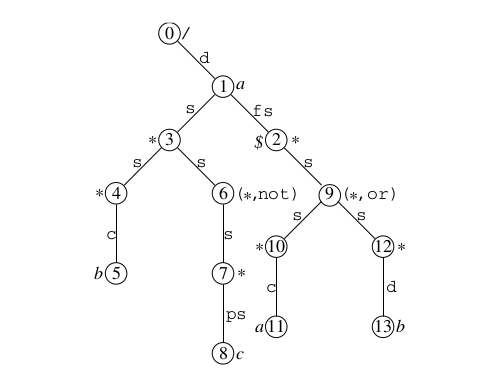
\includegraphics[scale=.5]{querytree.png}
\caption{Albero della query Q}
\end{figure}
Partendo da una query CXPath o un suo sottoinsieme è possibile costruire un albero Q della query; in figura è mostrato l'albero che corrisponde alla query 
\texttt{Q = /d::$a$[c::$b$ and not ps::$c$]/fs::*[c::$a$ or d::$b$]} dove con d si intende l'asse descendant::, con c l'asse child, con ps l'asse preceding-sibling, con fs l'asse following-sibling.\\
Nell'albero della query ogni nodo ha un etichetta con il tipo e l'eventuale operatore \texttt{bool}. A ogni arco è associato un asse.\\
Per prima cosa si costruisce un percorso lineare, detto trunk(Q) ignorando tutti i predicati dalla query.  ogni vertice di trunk(Q) corrisponde a un location step della query. L'ultimo nodo è contrassegnato con \$ è corrisponde al nodo di output della query.\\
I predicati possono essere ora aggiunti in maniera ricorsiva aggiungendo un arco con asse \texttt{self::} collegato al sotto albero del predicato; questo sottoalbero ha come radice un nodo di tipo * con l'eventuale operazione booleana (\texttt{and} può essere sottointesa). Viene creato un ramo per ogni operando che viene valutato ricorsivamente.
\\\\
Ramanan dimostra due importanti risultati:
\begin{itemize}
\item Valutare un espressione di $CXPath^+$ equivale a calcolare la simulazione del grafo della query Q rispetto al grafo del documento D
\item L'indice basato sulla simulazione è il più piccolo indice in grado di coprire le query di tipo $BPQ^+$
\end{itemize}
Il secondo risultato è interessante in quanto è noto che gli indici basati su bisimulazione preservano il linguaggio delle $BPQ$ ma nel caso in cui si incontrano query che non fanno uso dell'operatore not è possibile sfruttare la riduzione spaziale offerta dagli indici basati su simulazione.
